\definecolor{okblue}{HTML}{0072B2}\definecolor{okorange}{HTML}{E69F00}\definecolor{okverm}{HTML}{D55E00}\definecolor{okgrey}{HTML}{999999}
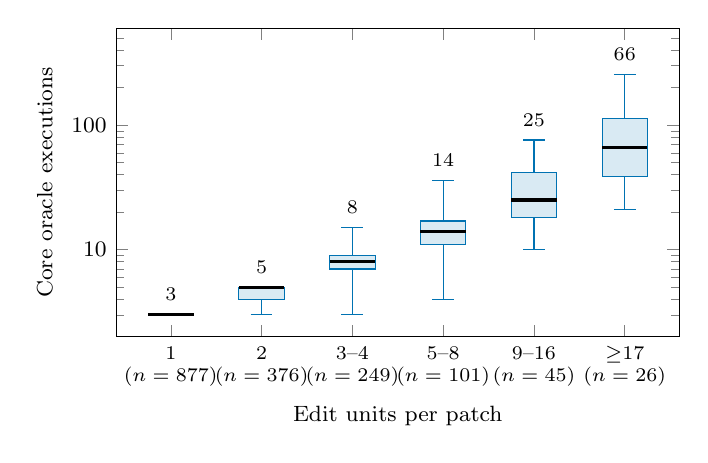
\begin{tikzpicture}
\begin{semilogyaxis}[width=0.72\linewidth,height=55mm,xmin=0.4,xmax=6.6,ymin=2,ymax=600,
 xtick={1,2,3,4,5,6},xticklabels={{1\\($n=877$)},{2\\($n=376$)},{3--4\\($n=249$)},{5--8\\($n=101$)},{9--16\\($n=45$)},{$\geq$17\\($n=26$)}},
 xticklabel style={align=center,font=\scriptsize},yticklabel style={font=\footnotesize},
 xlabel={Edit units per patch},ylabel={Core oracle executions},label style={font=\footnotesize},
 log ticks with fixed point,clip=false]
\addplot[draw=none] coordinates {(1,3)};
\draw[okblue] (axis cs:1,3) -- (axis cs:1,3);
\draw[okblue] (axis cs:1,3) -- (axis cs:1,3);
\draw[okblue] (axis cs:0.88,3) -- (axis cs:1.12,3);
\draw[okblue] (axis cs:0.88,3) -- (axis cs:1.12,3);
\draw[okblue,fill=okblue!15] (axis cs:0.75,3) rectangle (axis cs:1.25,3);
\draw[black,line width=1.2pt] (axis cs:0.75,3) -- (axis cs:1.25,3);
\node[font=\scriptsize,anchor=south] at (axis cs:1,3.24) {3};
\draw[okblue] (axis cs:2,3) -- (axis cs:2,4);
\draw[okblue] (axis cs:2,5) -- (axis cs:2,5);
\draw[okblue] (axis cs:1.88,3) -- (axis cs:2.12,3);
\draw[okblue] (axis cs:1.88,5) -- (axis cs:2.12,5);
\draw[okblue,fill=okblue!15] (axis cs:1.75,4) rectangle (axis cs:2.25,5);
\draw[black,line width=1.2pt] (axis cs:1.75,5) -- (axis cs:2.25,5);
\node[font=\scriptsize,anchor=south] at (axis cs:2,5.4) {5};
\draw[okblue] (axis cs:3,3) -- (axis cs:3,7);
\draw[okblue] (axis cs:3,9) -- (axis cs:3,15);
\draw[okblue] (axis cs:2.88,3) -- (axis cs:3.12,3);
\draw[okblue] (axis cs:2.88,15) -- (axis cs:3.12,15);
\draw[okblue,fill=okblue!15] (axis cs:2.75,7) rectangle (axis cs:3.25,9);
\draw[black,line width=1.2pt] (axis cs:2.75,8) -- (axis cs:3.25,8);
\node[font=\scriptsize,anchor=south] at (axis cs:3,16.2) {8};
\draw[okblue] (axis cs:4,4) -- (axis cs:4,11);
\draw[okblue] (axis cs:4,17) -- (axis cs:4,36);
\draw[okblue] (axis cs:3.88,4) -- (axis cs:4.12,4);
\draw[okblue] (axis cs:3.88,36) -- (axis cs:4.12,36);
\draw[okblue,fill=okblue!15] (axis cs:3.75,11) rectangle (axis cs:4.25,17);
\draw[black,line width=1.2pt] (axis cs:3.75,14) -- (axis cs:4.25,14);
\node[font=\scriptsize,anchor=south] at (axis cs:4,38.88) {14};
\draw[okblue] (axis cs:5,10) -- (axis cs:5,18);
\draw[okblue] (axis cs:5,42) -- (axis cs:5,76);
\draw[okblue] (axis cs:4.88,10) -- (axis cs:5.12,10);
\draw[okblue] (axis cs:4.88,76) -- (axis cs:5.12,76);
\draw[okblue,fill=okblue!15] (axis cs:4.75,18) rectangle (axis cs:5.25,42);
\draw[black,line width=1.2pt] (axis cs:4.75,25) -- (axis cs:5.25,25);
\node[font=\scriptsize,anchor=south] at (axis cs:5,82.08) {25};
\draw[okblue] (axis cs:6,21) -- (axis cs:6,38.75);
\draw[okblue] (axis cs:6,113.25) -- (axis cs:6,256);
\draw[okblue] (axis cs:5.88,21) -- (axis cs:6.12,21);
\draw[okblue] (axis cs:5.88,256) -- (axis cs:6.12,256);
\draw[okblue,fill=okblue!15] (axis cs:5.75,38.75) rectangle (axis cs:6.25,113.25);
\draw[black,line width=1.2pt] (axis cs:5.75,66) -- (axis cs:6.25,66);
\node[font=\scriptsize,anchor=south] at (axis cs:6,276.48) {66};
\end{semilogyaxis}
\end{tikzpicture}
